% codigoFuenteLibroR2
% Copyright (C) 2020  J.M. Perez Zerpa, et. al.
%
% This program is free software: you can redistribute it and/or modify
% it under the terms of the GNU General Public License as published by
% the Free Software Foundation version 3 of the License.
%
% This program is distributed in the hope that it will be useful,
% but WITHOUT ANY WARRANTY; without even the implied warranty of
% MERCHANTABILITY or FITNESS FOR A PARTICULAR PURPOSE. See the
% GNU General Public License for more details.
%
% You should have received a copy of the GNU General Public License
% along with this program.  If not, see <http://www.gnu.org/licenses/>.

\chapter[Método de Desplazamientos en pórticos]{Método de Desplazamientos en pórticos}

% intro e hipotesis
En esta Unidad Temática se presentan métodos de análisis de estructuras planas de barras en base a desplazamientos como incógnita principal. %
%
El enfoque adoptado para presentar el tema es similar al utilizado en \citep{Pilkey2002,Wunderlich2002}, utilizando los principios energéticos ya vistos en la Unidad Temática 2 de forma similar a como es realizado en \citep{Reddy2002b}.
% ----------------------------




\section{Teoría de vigas sometidas a flexión compuesta} \label{sec:teoviga}

\subsection{Hipótesis y definiciones fundamentales}

Para el análisis de pórticos es necesario abordar el estudio de vigas sometidas a cargas transversales y axiales, esto será llamado \textit{flexión compuesta}. %
%
Para esto, un posible camino es agregar el efecto de la directa a las ecuaciones de la teoría de vigas a flexión pura, presentadas en la sección \ref{sec:teovigastimo}. %
%
Sin embargo se optará por otro camino orientado a deducir las ecuaciones a partir de algunas hipótesis de la teoría de vigas integradas con la Teoría de la Elasticidad. %
%
Este enfoque es utilizado en literatura de referencia \citep{Wunderlich2002,Onate2013} y permite llegar a los mismos resultados.

\subsubsection{Hipótesis}
Sea el campo de desplazamientos de los puntos de la viga, dados por el vector formado por las funciones: $u(x,y,z)$, $v(x,y,z)$ y $w(x,y,z)$, representando desplazamientos en $x$, $y$ y $z$ respectivamente. %
%
Asumiendo que la flexión se produce en el plano $x-y$, se consideran las siguientes hipótesis:
%
\begin{enumerate}
	\item Los desplazamientos transversales (flecha) de todos los puntos en una sección transversal (ubicada en la coordenada $x$)  son pequeños e iguales al desplazamiento del eje de la viga.
	$$
	v(x,y,z) =  v(x).
	$$
	\item Las secciones transversales permanecen planas y perpendiculares al eje deformado durante la deformación y los giros $\theta$ son pequeños. %
	%
	Los desplazamientos axiales por tanto están dados por:
	\begin{equation} \label{eqn:despaxi}
	u(x,y,z) = u_G(x) - y \theta(x),
	\end{equation}
	donde $\theta$ es el ángulo que forma el vector tangente de la curva de la deformada del eje con la horizontal y $u_G(x)$ es la función del desplazamiento axial del baricentro de la sección ubicada en $x$. 
	%
	\item Todos los desplazamientos perpendiculares al plano de deformación de la viga son nulos
$$
w(x,y,z) = 0
$$
	%
	\item Se asume que no existen esfuerzos aplicados perpendiculares al plano de deformación de la viga
	\item Se desprecia la energía de deformación por cortante es decir, la distorsión angular.
\end{enumerate}

Respecto a la hipótesis de desplazamientos perpendiculares al plano, esta hipótesis representa una simplificación del comportamiento real de la estructura y el efecto de Poisson, sin embargo simplifica la aplicación de la ecuación constitutiva y el cálculo del tensor de deformaciones y permite llegar a las ecuaciones de la teoría de vigas de forma directa.

Respecto a la no consideración de energía de deformación por cortante, se recomienda al estudiante interesado libros como \citep{Onate2013} donde se describen los elementos de viga de Timoshenko o  artículos recientes en los que se muestra la utilidad de este tipo de enfoques para simular el comportamiento real de estructuras \citep{Bui2014}. %
%
En este curso no se considerará deformación por cortante, hipótesis que puede ser razonable para vigas cuya relación entre largo y altura de sección transversal sea superior a 10: $L/h > 10$ (este número es adoptado como criterio para este curso, otros estudios numérico/experimentales pueden sugerir otros valores).

\subsubsection{Tensor de deformaciones}

Se comienza calculando las componentes del tensor de deformaciones aplicando la relación desplazamientos-deformación al campo de desplazamientos considerado (ver Ecuación~\eqref{eqn:despaxi}). %
%
La deformación axial  $\varepsilon_x$ está dada por:
%
\begin{equation}\label{eqn:expdef}
\varepsilon_x(x,y) =  \varepsilon_G (x) -y \frac{\partial \theta}{\partial x}(x).
\end{equation}
%
donde $\varepsilon_G$ es la deformación axial del eje de la viga, y está dada por
%
\begin{equation}
\varepsilon_G(x) =  \frac{\partial u_G}{\partial x} (x) .
\end{equation}


La distorsión angular $\gamma_{xy}$ está dada por:
\begin{equation}
  \gamma_{xy}(x,y) = -\theta(x) + \frac{\partial v}{\partial x} (x).
\end{equation}
%
La no dependencia de $\gamma_{xy}$ respecto a $y$ implica que la cara permanece plana. %
%
Al imponer que la distorsión angular (asociada a la deformación por cortante) sea nula, se aporta la condición:
\begin{equation}
\boxed{
\theta = \frac{\partial v}{\partial x},
}
\end{equation}
lo que es equivalente a que la normal a la sección transversal deformada coincida con la tangente a la curva deformada.

Finalmente la expresión de la deformación axial está dada por:
%
\begin{equation}\label{eqn:epsdef}
\boxed{
\varepsilon_x(x,y) =  \varepsilon_G (x) -y \frac{\partial^2 v}{\partial x^2}(x).
}
\end{equation}
lo que representa una extensión de la expresión obtenida en la Ecuación~\eqref{eqn:epstimo} para el caso de deformación axial.

\cajaactividad{
Demostrar que, considerando las hipótesis de desplazamiento mencionadas, la única componente del tensor de deformaciones no nula, es $\varepsilon_{xx}$.
}



\subsubsection{Tensor de tensiones}

Se considera que el material es elástico lineal e isótropo. Se utiliza la correspondiente ecuación constitutiva y el tensor de deformaciones obtenido, teniendo la relación:
%
\begin{equation}
  \sigma_x = E \varep_x
\end{equation}

Esta componente de $\bfsig$ es la única que produce trabajo interno en la expresión de la energía interna de deformación dada por la Ecuación~\eqref{eqn:energbarra}.

\subsection{Solicitaciones y convenciones de signo}


\subsubsection{Solicitaciones internas}

Se definen las solicitaciones internas correspondientes a la tensión axial: directa y momento. %
%
Para la directa se tiene
%
\begin{equation}
N (x) = \int_{A(x)} \sigma_x (x,y) \, \dif A
\end{equation}
%
usando que la sección transversal es uniforme, la ecuación constitutiva y la expresión de la deformación axial se tiene:
%
\begin{equation}
N (x) = \int_{A(x)} \left( E \frac{\partial u_G}{\partial x} - E y \frac{\partial^2 v}{\partial x^2}   \right) \, \dif A.
\end{equation}
%
Usando que el vector $\bfe_x$ pasa por el punto $G$, baricentro de la sección transversal, se tiene
%
\begin{equation}\label{eqn:direc}
\boxed{
N (x) =  E A  \varepsilon_G(x).
}
\end{equation}
%
Se puede destacar que la convención de signo de directa positiva a tracción es coherente con el resultado obtenido ya que en dicho caso $\varepsilon_G >0$.

Para el cálculo del momento según el eje $\bfe_z$ se considera la suma (integral) del momento de diferenciales de área por su brazo respectivo:
%
\begin{equation}
M_z (x) = \int_{A(x)} \left( y \bfe_y \,  \wedge \, \sigma_x (x,y) \bfe_x \right) \cdot \bfe_z \dif A.
\end{equation}
%
Sustituyendo las expresiones de las tensiones y la deformación dada por la Ecuación~\eqref{eqn:expdef} se obtiene:
%
\begin{equation}
M_z (x) = \int_{A(x)} y E \varep_{G} \left( \bfe_y \,  \wedge \, \bfe_x \right) \cdot \bfe_z \dif A + \int_{A(x)} -y^2 \frac{\partial^2 v}{\partial x^2} (x)  \left( \bfe_y \,  \wedge \, \bfe_x \right) \cdot \bfe_z \dif A.
\end{equation}

Calculando el producto mixto y usando que el primer momento de inercia respecto al baricentro es nulo, se obtiene:
%
\begin{equation}
M_z (x) = E \int_{A(x)} y^2 \dif A \,  \frac{\partial^2 v}{\partial x^2} (x)
\end{equation}
%
usando que el material tiene sección transversal uniforme y definiendo el segundo momento de inercia respecto de $z$ como $I_z(x) = \int_{A} y^2 dA$ se obtiene:
%
\begin{equation}\label{eqn:momen}
\boxed{
M_z (x) = E I_z \frac{\partial^2 v}{\partial x^2}(x).
}
\end{equation}

Por simplicidad de notación, a continuación se omitirán los subíndices $z$ y el argumento $x$. %
%
Esta notación con subíndices volverá a ser utilizada al considerar problemas de flexión esviada.

La relación obtenida entre momento y curvatura es muy relevante para la caracterización del comportamiento de estructuras de vigas incluso cuando el comportamiento incluye fenómenos complejos como fisuración y otras no linealidades.


\subsubsection{Expresión de tensión axial en función de solicitaciones}


%
A partir de la expresiones de la directa, dada por la Ecuación~\eqref{eqn:direc}, y del momento, dado por la Ecuación~\eqref{eqn:momen}, se obtiene:
%
\begin{equation}
\varepsilon_G(x) = \frac{	N (x) }{E A}
\qquad
\frac{\partial^2 v}{\partial x^2}(x) = \frac{	M_z (x) }{E I_z} 
\end{equation}
%
Sustituyendo en la expresión de la deformación axial dada por la Ecuación~\eqref{eqn:epsdef} se obtiene:
%
\begin{equation}
\varepsilon_x(x,y) = \frac{	N (x) }{E A}  -y  \frac{ M_z (x) }{E I_z},
\end{equation}

y multiplicando por $E$ ambos miembros y usando la ecuación constitutiva se tiene
%
\begin{equation}
\boxed{
\sigma(x,y) = \frac{	N (x) }{A}
- y \frac{	M_z (x) }{I_z} 
}
\end{equation}


\subsubsection{Convenciones de signo}

Para el desarrollo de métodos de análisis de pórticos es útil y necesario definir una convención de signos diferente a la usada para las solicitaciones internas. %
%
En la \autoref{fig:conve} se muestran dos convenciones de signo a ser utilizadas en este documento y en todo el curso.
%
\begin{figure}[htb]
  \centering
  \def\svgwidth{0.8\textwidth}
  \input{figs/UT3/convenciones_signos_vigas.pdf_tex}
	\caption{Convenciones de signo para momentos nodales y cargas externas en coordenadas locales.}
	\label{fig:conve}
\end{figure}

Las \textbf{solicitaciones internas} definidas con la convención de signos usual para $\sigma$ (positivo tracción) corresponden a la convención de signos \textbf{1} de la figura. %
%
Esta convención corresponde a aquella en la cual momentos positivos representan una tracción de fibras inferiores.

Por otra parte, la convención \textbf{2} es útil para el desarrollo de métodos matriciales o computacionales, asociada a las \textbf{fuerzas externas} aplicadas.

\subsubsection{Ecuaciones de equilibrio}

Las ecuaciones para vigas sometidas a cargas transversales $q$ y axiales $b$ distribuidas por unidad de longitud están dadas por:
%
\begin{eqnarray}
\frac{dN}{dx}(x) & =& -b(x) \\
\frac{dV}{dx}(x) & =& q(x) \label{eqn:eqcortante}\\
\frac{\partial M}{\partial x}(x) & =& V(x)
\end{eqnarray}
%

La deducción de estas ecuaciones a partir del equilibrio de un segmento diferencial fue realizado en cursos anteriores. %
Por otra parte, este desarrollo también puede ser realizado a partir del teorema de trabajo virtual, de forma similar a como es hecho en la sección 5.4.5 de \citep{Hughes1987a}.


\subsection{Relaciones fuerzas-desplazamientos para vigas a flexión}\label{sec:mdvig}

Se considera una viga de largo $L$, formada por un material de módulo de Young $E$ y con sección transversal uniforme de inercia $I$ sometida a fuerzas aplicadas en los extremos de \textbf{cortante y momento} de acuerdo a la convención 2 de la \autoref{fig:conve}. %
%
Se asume que no hay cargas aplicadas en el tramo intermedio de la viga, ni distribuidas ni puntuales. %
%

Se considera que no hay deformación axial o esta es despreciable ($\varep_{G}\approx 0$). %
%
También se omitirá el sub-índice $z$ en $M_z$ y $\theta_z$. 

\subsubsection{Ecuación de la elástica}

A partir de las ecuaciones de equilibrio y la ecuación de la elástica se obtiene que la flecha es una función de tercer grado, por lo que se considera la siguiente expresión polinómica general:
%
\begin{equation}\label{eqn:ecw}
v(x) = a_3 x^3 + a_2 x^2 + a_1 x + a_0, \qquad \forall x \in [0,L].
\end{equation}

En lugar de trabajar con los parámetros $a_i$ se desea representar la función $v$ en función de los valores nodales de flecha y giro, es decir, $v_1$,  $\theta_1$, $v_2$ y $\theta_2$. %
%
Para esto, se plantean las siguientes relaciones entre la flecha $v$ evaluada en ciertos puntos en particular y los desplazamientos nodales:
%
\begin{equation}
v_1 = v(0), \qquad
\theta_1 = \frac{d v}{d x} (0), \qquad
v_2 = v(L), \qquad
\theta_2 = \frac{d v}{d x}(L).
\end{equation}

Resolviendo el sistema de ecuaciones lineales se obtiene:
%
\begin{eqnarray}
a_3 &=& \frac{1}{L^3} \left( \theta_{1} L + \theta_{2} L + 2 v_{1} - 2 v_{2} \right) \nonumber\\
a_2 &=&	\frac{1}{L^2} \left( - 2 \theta_{1} L - \theta_{2}  L - 	3 v_{1} + 3 v_{2}  \right) \nonumber\\
a_1 &=&	\theta_{1} \nonumber\\
a_0 &=&	v_{1}, \nonumber
\end{eqnarray}
%
y sustituyendo en la Ecuación~\eqref{eqn:ecw} se obtiene la expresión:
%
\begin{equation} \label{eqn:elastica}
v(x) =  \varphi_{v_1}(x) v_1 + \varphi_{\theta_1}(x) \theta_1
+ \varphi_{v_2}(x) v_2 + \varphi_{\theta_2}(x) \theta_2,
\end{equation}
%
donde las funciones $\varphi$ son funciones de interpolación dadas por:
%
\begin{eqnarray}
\varphi_{v_1} (x) &=& \left(1 - \frac{3 x^{2}}{L^{2}} + \frac{2 x^{3}}{L^{3}}\right) \\
\varphi_{\theta_1} (x) &=&	\left(x - \frac{2 x^{2}}{L} + \frac{x^{3}}{L^{2}}\right) \\
\varphi_{v_2} (x) &=&	\left(\frac{3 x^{2}}{L^{2}} - \frac{2 x^{3}}{L^{3}}\right) \\
\varphi_{\theta_2} (x) &=& \left(- \frac{x^{2}}{L} + \frac{x^{3}}{L^{2}}\right) .
\end{eqnarray}

En la \autoref{fig:phis} se muestran los gráficos de las funciones de interpolación, los cuales corresponden a las funciones de las elásticas para desplazamientos o giros unitarios de cada grado de libertad correspondiente. %
%

%
\begin{figure}[htb]
	\centering
	\subfloat[Funciones de interpolación $\varphi_{v_1}$ y $\varphi_{v_2}$.]{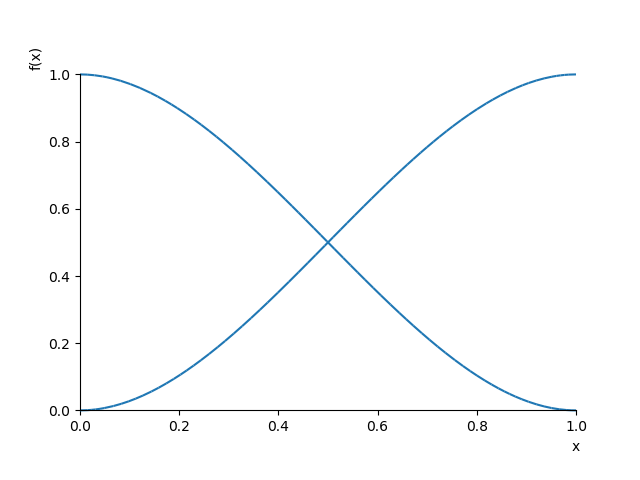
\includegraphics[width=0.47\textwidth]{phisv}\label{fig:phiv}}
	\subfloat[Funciones de interpolación $\varphi_{\theta_1}$ y $\varphi_{\theta_2}$.]{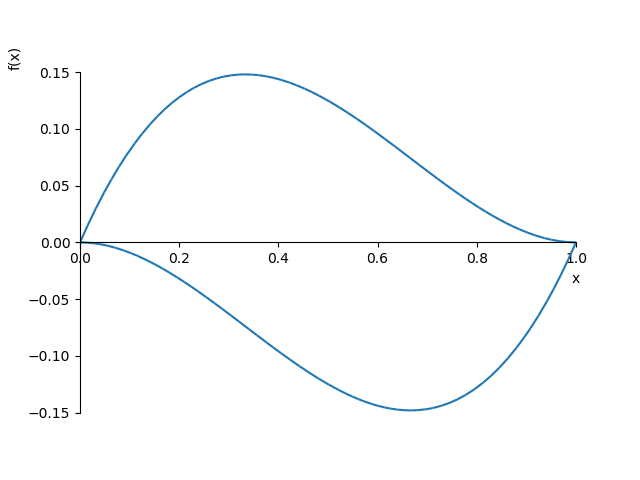
\includegraphics[width=0.47\textwidth]{phist}\label{fig:phit}}
	\caption{Gráfico de funciones de interpolación para $L=1$.}
	\label{fig:phis}
\end{figure}




\subsubsection{Mínima energía potencial y teorema de Castigliano}


Se tiene entonces definidas las funciones de interpolación $\phi$ definidas al inicio de la UT2, correspondientes al caso de vigas a flexión pura.
%
Se tiene también las expresiones de la deformación axial y la ecuación constitutiva por lo que se está en condiciones de aplicar el principio de mínima energía potencial. Aplicando el principio se obtendrán las relaciones entre fuerzas y desplazamientos para las cuales se cumplen con ecuaciones de compatibilidad de desplazamientos y equilibrio con fuerzas externas.

Dado que se desprecia la energía de deformación por cortante (asociada al producto $\tau_{xy} \gamma_{xy}$), la energía potencial de deformación de la viga está dada por:
%
\begin{equation}
\Pi_{int} = \frac{1}{2} \int_\Omega \bfsig : \bfvarep  \dif V  = \frac{1}{2} \int_\Omega \sigma_x \varepsilon_x  \dif V. 
\end{equation}

Sustituyendo las ecuaciones \eqref{eqn:eccons} y \eqref{eqn:expdef} y usando que se desprecia la deformación axial $\varep_G$ se tiene:
%
\begin{equation}\label{eqn:ut3piviga}
\Pi_{int} = \frac{1}{2} \int_0^L \int_{A(x)} E y^2 \left( \frac{\partial^2 v}{\partial x^2}\right)^2  \dif A \dif x 
=  E I  \frac{1}{2} \int_0^L \left( \frac{\partial^2 v}{\partial x^2}\right)^2 \dif x .
\end{equation}

%
Se destaca que fue despreciada la energía de deformación axial por directas (en caso de que fueran aplicadas) es decir que el término $EA\varepsilon_G^2$ se consideró mucho menor que $EI \kappa^2$.

Usando la Ecuación~\eqref{eqn:elastica} se obtiene la energía de deformación en función de los desplazamientos y giros nodales $\Pi_{int}(v_1,\theta_1,v_2,\theta_2)$.

Para este desarrollo se considera la convención de signos 2 tanto para fuerzas y momentos como para desplazamientos. %
%
De esta forma la energía potencial de las fuerzas externas está dada por:
\begin{equation}
\Pi_{ext}(v_1,\theta_1,v_2,\theta_2) = - F_{y,1} v_1 - M_1 \theta_1  - F_{y,2} v_2 - M_2 \theta_2,
\end{equation}
%
y por lo tanto, la energía potencial total está dada por:
\begin{equation}
\Pi(v_1,\theta_1,v_2,\theta_2) =  \Pi_{int}(v_1,\theta_1,v_2,\theta_2)  - F_{y,1} v_1 - M_1 \theta_1 - F_{y,2} v_2 - M_2 \theta_2,
\end{equation}

Las condiciones de mínima energía potencial total pueden por lo tanto ser escritas como:
%
\begin{eqnarray}
\frac{\partial \Pi_{int}}{\partial v_1}(v_1,\theta_1,v_2,\theta_2) &=&  F_{y,1} \\
\frac{\partial \Pi_{int}}{\partial \theta_1}(v_1,\theta_1,v_2,\theta_2) &=&  M_1 \label{eqn:ut3castm1} \\
\frac{\partial \Pi_{int}}{\partial v_2}(v_1,\theta_1,v_2,\theta_2) &=&  F_{y,2} \\
\frac{\partial \Pi_{int}}{\partial \theta_2}(v_1,\theta_1,v_2,\theta_2) &=&  M_2
\end{eqnarray}


A modo de ejemplo se presenta el desarrollo para la condición del momento del nodo izquierdo, es decir, la Ecuación~\eqref{eqn:ut3castm1}. %
%
Usando la interpolación de la flecha en la Ecuación~\eqref{eqn:ut3piviga} y calculando la derivada, se tiene:
%
\begin{equation}
\frac{\partial \Pi_{int}}{\partial \theta_1} = \frac{1}{2} EI \int_0^{L} 2 \left( \frac{\partial^2 v}{\partial x^2} (v_1,\theta_1,v_2,\theta_2) \varphi_{\theta_1}'' \right) \dif x
\end{equation}
%
para evaluar la derivada de $v$ se utilizan las expresiones de las derivadas de las funciones de interpolación dadas por:
%
\begin{eqnarray}
	\varphi_{v_1}'' (x) = \left(- \frac{6}{L^{2}} + \frac{12 x}{L^{3}}\right) \qquad %
	\varphi_{\theta_1}'' (x) =	\left( - \frac{4}{L} + \frac{6 x }{L^{2}}\right) \\
	\varphi_{v_2}'' (x) =	\left(\frac{6}{L^{2}} - \frac{12 x}{L^{3}}\right) \qquad %
	\varphi_{\theta_2}'' (x) = \left(- \frac{2}{L} + \frac{6 x}{L^{2}}\right) .
\end{eqnarray}
%
sustituyendo $v$ por la expresión dada por las funciones de interpolación se obtiene:
%
\begin{equation}
\frac{\partial \Pi_{int}}{\partial \theta_1} = K_{v_1,\theta_1} v_1 + K_{\theta_1,\theta_1} \theta_1 + K_{v_2,\theta_1} v_2  + K_{\theta_2,\theta_1} \theta_2
\end{equation}
%
donde los coeficientes $K$ están dados por las integrales:
%
\begin{eqnarray}
K_{v_1,\theta_1} = EI \int_0^L \varphi_{v_1}'' \varphi_{\theta_1}'' \dif x \qquad
%
K_{\theta_1,\theta_1} = EI \int_0^L \varphi_{\theta_1}'' \varphi_{\theta_1}'' \dif x \\
%
K_{v_2,\theta_1} = EI \int_0^L \varphi_{v_2}'' \varphi_{\theta_1}'' \dif x \qquad 
%
K_{\theta_2,\theta_1} = EI\int_0^L \varphi_{\theta_2}'' \varphi_{\theta_1}'' \dif x 
\end{eqnarray}
%
Calculando las integrales se tiene:
%
\begin{eqnarray}
K_{v_1,\theta_1} &=& EI \left(   \frac{24}{L^2} -  \frac{84}{2} \frac{1}{L^2} + \frac{72}{3} \frac{1}{L^2} \right) = EI \frac{6}{L^2} \\
%
K_{\theta_1,\theta_1} &=& EI \left(   \frac{16}{L^2} -  \frac{48}{2}\frac{1}{L^2} +\frac{36}{3} \frac{1}{L^2}  \right) L = EI \frac{4}{L}\\
%
K_{v_2,\theta_1} &=& EI \left(  - \frac{24}{L^2} + \frac{84}{2} \frac{1}{L^2} - \frac{72}{3} \frac{1}{L^2} \right) = -EI \frac{6}{L^2} \\
%
K_{\theta_2,\theta_1} &=& EI \left(   \frac{8}{L^2} -  \frac{36}{2} \frac{1}{L^2} + \frac{36}{3} \frac{1}{L^2}  \right)L = EI \frac{2}{L}
\end{eqnarray}

Se obtiene por lo tanto que la ecuación de Castigliano para el giro del primer nodo, dada por la Ecuación~\eqref{eqn:ut3castm1}, puede ser escrita como:
%
\begin{equation}
EI \frac{6}{L^2} v_1 +  EI \frac{4}{L} \theta_1 - EI \frac{6}{L^2} v_2 +    EI \frac{2}{L} \theta_2 = M_1.
\end{equation}


Repitiendo el procedimiento para las otras condiciones de Castigliano se llega a:
%
\begin{eqnarray}
EI \left( \dfrac{12}{L^{3}} v_1 + \dfrac{6}{L^{2}} \theta_1 - \dfrac{12}{L^{3}} v_2 + \dfrac{6}{L^{2}} \theta_2 \right)  &=& F_{y,1} \\
EI \left( \frac{6}{L^2} v_1 +  \frac{4}{L} \theta_1 - \frac{6}{L^2} v_2   + \frac{2}{L} \theta_2 \right) &=& M_1 \\
EI \left( -\dfrac{12}{L^{3}} v_1 - \dfrac{6}{L^{2}} \theta_1 +\dfrac{12}{L^{3}} v_2 - \dfrac{6}{L^{2}} \theta_2 \right) &=& F_{y,2} \\
EI \left( \dfrac{6}{L^{2}} v_1 + \dfrac{2}{L} \theta_1 - \dfrac{6}{L^{2}} v_2 + \dfrac{4}{L}  \theta_2 \right) &=& M_2,
\end{eqnarray}
%

Estas ecuaciones representan un sistema de ecuaciones cuyas incógnitas son los desplazamientos y giros y el dato o término independiente son las fuerzas. %
%
Estas relaciones pueden ser escritas en forma matricial como
\begin{equation}
\bfK \bfu = \bff	
\end{equation}
%
donde
\begin{equation}
\bfK =  EI \left[
\begin{matrix}
\dfrac{12}{L^{3}}  & \dfrac{6}{L^{2}} & - \dfrac{12}{L^{3}} & \dfrac{6}{L^{2}} \\[3mm]
\dfrac{6}{L^2}  & \dfrac{4}{L} & - \dfrac{6}{L^2} & \dfrac{2}{L}  \\[3mm]
-\dfrac{12}{L^{3}} & - \dfrac{6}{L^{2}} & \dfrac{12}{L^{3}} & - \dfrac{6}{L^{2}} \\[3mm]
\dfrac{6}{L^{2}} & \dfrac{2}{L} & - \dfrac{6}{L^{2}} & \dfrac{4}{L} 
\end{matrix}
\right]
\quad \text{y}\quad
\bff =  \left[
\begin{matrix}
F_{y,1} \\[3mm]
M_{1} \\[3mm]
F_{y,2} \\[3mm]
M_{2} \\
\end{matrix}
\right]
\end{equation}



%
Es importante destacar qué condiciones de contorno (en los desplazamientos) deben ser aplicadas para poder obtener una solución única, es decir, eliminar los posibles movimientos de cuerpo rígido que tenga la viga.



\cajaactividad{
Calcular la flecha máxima de una viga de largo $\ell$, biempotrada, con rigidez flexional uniforme $E I$ y una carga puntual $P$ aplicada en la mitad de su longitud, usando el método de los desplazamientos en su forma matricial, utilizando dos elementos.
}


%\subsection{Ejemplo}

%\subsection{Principio de trabajos virtuales}

%El principio de trabajos virtuales establece que la elástica de equilibrio $w(x)$ será aquella que cumpla que
%%
%\begin{equation}
%EI \int_{0}^{L} \frac{d^2 w}{d x^2} \, \frac{d^2 \tilde{w} }{d x^2} \, \dif x = V_1 \tilde{w}_1 +  M_1 \tilde{\theta}_1 + V_2 \tilde{w}_2 + M_2 \tilde{\theta}_2
%\end{equation}
%



\section{Métodos de analíticos para pórticos}


\subsection{Ecuaciones para métodos analíticos}

Los métodos analíticos de resolución se basan en el planteo de las ecuaciones para cada elemento de la estructura independientemente e imponer condiciones de equilibrio en los nodos de unión correspondientes. %
%
Para aplicar estos métodos es conveniente definir variables auxiliares como $\psi$, dada por la expresión:
%
\begin{equation}
  \psi = \frac{v_2 - v_1}{L}.
\end{equation}
%

$\psi$ puede ser interpretado geométricamente como el giro antihorario (en pequeños giros) de la recta que une los dos nodos (cuerda). Se puede ver un diagrama en la \autoref{fig:psi}.

\begin{figure}[htb]
	\centering
	\def\svgwidth{0.65\textwidth}
	\input{figs/UT3/diagramaPsi.pdf_tex}
	\caption{Diagrama para interpretación geométrica de $\psi$.}
	\label{fig:psi}
\end{figure}


Las ecuaciones de Castigliano asociadas a los momentos pasan a ser: %
%
\begin{equation}\label{eqn:eqvig}
\left\{
\begin{array}{rl}
\displaystyle
\frac{2 EI}{L} \left( 2 \theta_1  + \theta_2 - 3 \psi   \right) =& M_1 \\[3mm]
\displaystyle
\frac{2 EI}{L} \left( \theta_1 + 2  \theta_2 - 3 \psi  \right) =& M_2
\end{array}
\right.
\end{equation}

Por otra parte a partir de combinaciones lineales de las ecuaciones de momento y cortante se obtiene las relaciones:
%
\begin{equation}
\left\{
\begin{array}{rl}
\displaystyle
F_{y,1} & \displaystyle
 = \frac{M_1 + M_2}{L} \\[5mm]
\displaystyle
F_{y,2} & \displaystyle
 = -\frac{M_1 + M_2}{L} 
\end{array}
\right.
\end{equation}

Estas ecuaciones son planteadas para cada elemento de barra y los momentos que actúan sobre cada nodo son considerados en ecuaciones de equilibrio nodal, obteniendo así el número de ecuaciones necesarias para obtener todos los desplazamientos y giros.




\subsection{Cargas equivalentes} \label{sec:cargequiv}

En el caso en que la barra tenga cargas aplicadas entre los nodos se puede considerar fuerzas y momentos aplicados en los nodos con la misma energía potencial externa. %
%
Estas fuerzas nodales son llamadas cargas equivalentes. %
%
Este método permite obtener valores exactos de giros y flechas nodales, sin embargo, es necesario integrar las ecuaciones de equilibrio para obtener los diagramas de solicitaciones  y elástica en el tramo.

%La energía potencial de las cargas aplicadas estas cargas es:
%
%\begin{equation}
%V_{ext}^{tr} = -\int_{0}^{L} q(x) v(x) \dif x - P v(x_P)
%\end{equation}
%
%nuevamente se utiliza la expresión de la elástica de la Ecuación~\eqref{eqn:elastica}. 

A continuación se consideran dos casos importantes de cargas en el tramo, con un enfoque como el presentado en \citep{Onate2013} donde se puede encontrar un desarrollo más completo. %

\subsubsection{Carga distribuida}

En el caso de carga distribuida $q(x)$ (de acuerdo a la convención 2), se tiene que la energía potencial de las fuerzas $\Pi^{tr}_{ext}$ está dada por:
%
\begin{equation}
\Pi_{ext}^{tr} =
- \int_0^L q(x) v(x) \dif x.
\end{equation}
%
El objetivo es entonces encontrar las fuerzas nodales equivalentes que tengan la misma energía potencial. Para esto se sustituye la expresión de $v(x)$ dada por la Ecuación~\eqref{eqn:elastica}, obteniendo:
%
\begin{equation}
\Pi_{ext}^{tr} =
-F_{y,1}^{tr} v_1 - M_1^{tr} \theta_1 -F_{y,2}^{tr} v_2 -  M_2^{tr} \theta_2
\end{equation}
donde
\begin{eqnarray}
F_{y,1}^{tr} = \int_{0}^{L} q(x) \varphi_{v_1}(x) \dif x \qquad & \displaystyle M_1^{tr} = \int_{0}^{L}q(x) \varphi_{\theta_1}(x)  \dif x  \nonumber\\
F_{y,2}^{tr} = \int_{0}^{L}q(x) \varphi_{v_2}(x)  \dif x \qquad & \displaystyle M_2^{tr} = \int_{0}^{L} q(x)\varphi_{\theta_2}(x)  \dif x  \nonumber
\end{eqnarray}

En el caso particular de carga distribuida uniforme $q(x) = q$ se tiene:
%
\begin{eqnarray}
F_{y,1}^{tr} &=& \frac{q L}{2} \\
M_1^{tr} &=& \frac{q L^{2}}{12} \\
F_{y,2}^{tr} &=& \frac{q L}{2} \\
M_2^{tr} &=& - \frac{q L^{2}}{12}
\end{eqnarray}

\cajaconcepto{Empotramiento perfecto}{
Es importante ver que estas fuerzas nodales corresponden a los valores opuestos a las reacciones de una viga biempotrada, también llamadas momentos de \textit{empotramiento perfecto} $M^{emp}$ y sus respectivas fuerzas verticales o de cortante $F_y^{emp}$. %
%
Los cortantes y momentos de empotramiento perfecto son opuestos a sus correspondientes fuerzas de tramo, es decir: $F_y^{emp} = -F_y^{tr}$ y $M^{emp} = -M^{tr}$.
}

\subsubsection{Carga puntual}

Se considera ahora que la carga puntual $P$ es aplicada (según la convención 2) en el punto de coordenada $x= x_P$ con $x_P \in (0,L)$ y que $q(x)=0$.

La energía potencial de la fuerza en el tramo está dada por:
%
\begin{equation}
\Pi_{ext}^{tr} = - P v (x_P) =  -P \varphi_{v_1}(x_P) v_1 - P \varphi_{\theta_1}(x_P) \theta_1
- P \varphi_{v_2}(x_P) v_2 - P \varphi_{\theta_2}(x_P) \theta_2,
\end{equation}
%
por lo tanto las fuerzas nodales equivalentes a la carga puntual en $x_P$ son calculadas evaluando las funciones $\varphi$. %
%
Por ejemplo el momento nodal en 1 es
%
\begin{equation}
M_1^{tr} = P \varphi_{\theta_1} (x_P) = P  \left(x_P - \frac{2 x_P^{2}}{L} + \frac{x_P^{3}}{L^{2}}\right)
\end{equation}
%
expresión que, factorizando, puede ser reescrita como:
\begin{equation}
M_1^{tr} = P x_P (L-x_P)^2 \frac{1}{L^2}.
\end{equation}
Se verifica nuevamente que el momento equivalente es el opuesto del momento de empotramiento perfecto.

Para el otro momento se tiene
\begin{equation}
M_2^{tr} = -P x_P^2 (L-x_P) \frac{1}{L^2},
\end{equation}
%
y para las cargas equivalentes se tiene
%
\begin{equation}
F_{y,1}^{tr} = P \left(1 - \frac{3 x^{2}}{L^{2}} + \frac{2 x^{3}}{L^{3}}\right) \qquad
F_{y,2}^{tr} =
P \left(\frac{3 x^{2}}{L^{2}} - \frac{2 x^{3}}{L^{3}}\right).
\end{equation}

%
%\subsection{Ejemplo}
%
%%Para verificar los valores de las fuerzas nodales para la carga puntual consideramos un problema con solución conocida. %
%%
%En clase se resolverá el problema de una ménsula de módulo de Young $E$ inercia $I$ y largo $L$ con una carga aplicada $P$ en $x_P$ como se muestra en la figura.
%\begin{center}
%	\setlength{\unitlength}{0.5\textwidth}
%	\begin{picture}(1,0.33597629)%
%	\put(0,0){\includegraphics[width=\unitlength,page=1]{mensula_carga_puntual_tramo.pdf}}%
%	\put(0.24867277,0.06426678){\color[rgb]{0,0,0}\makebox(0,0)[lb]{\smash{$x_P$}}}%
%	\put(0.49097862,0.25976283){\color[rgb]{0,0,0}\makebox(0,0)[lb]{\smash{$P$}}}%
%	\put(0,0){\includegraphics[width=\unitlength,page=2]{mensula_carga_puntual_tramo.pdf}}%
%	\end{picture}%
%\end{center}

%Sabemos que los desplazamiento y giro del extremo derecho son
%$$
%w_2 = - \frac{Px_P^2}{6 EI} (3 L -x_P) \qquad \theta_2 = -\frac{P x_P^2}{2 EI}
%$$
%
%Resolvemos ahora aplicando el método. El sistema de ecuaciones es
%
%\begin{eqnarray}
%EI \frac{12}{L^3} w_2 - EI \frac{6}{L^2} \theta_2 & = & -P \left( \frac{3 x_P^2}{L^2} - \frac{2 x_P^3}{L^3} \right) \nonumber\\
%EI \frac{-6}{L^2} w_2 + EI \frac{4}{L} \theta_2 & = & -P \left( -\frac{ x_P^2}{L} + \frac{x_P^3}{L^2} \right) \nonumber
%\end{eqnarray}
%
%multiplicando la segunda ecuación por $2/L$ y sumando la primera se tiene
%
%\begin{equation}
%EI \left(  \frac{-6}{L^2} + \frac{8}{L^2} \right) \theta_2 = -P \left( 3 \frac{ 3x_P^2}{L^2} - \frac{2 x_P^2}{L^2} -  \frac{2 x_P^3}{L^3} + \frac{2 x_P^3}{L^3}  \right)
%\end{equation}
%
%simplificando y despejando se llega a 
%
%\begin{equation}
%\theta_2 = -\frac{P x_P^2}{2 EI}
%\end{equation}
%
%sustituyendo en la primer ecuación se tiene
%
%\begin{equation}
%EI \frac{-6}{L^2} w_2 + EI\frac{4}{L} \left(-\frac{P x_P^2}{2 EI}\right) = -P \left(  \frac{-x_P^2}{L}  + \frac{x_P^3}{L^2} \right)
%\end{equation}
%
%simplificando y despejando se llega a
%
%\begin{equation}
%w_2 = - \frac{Px_P^2}{6 EI} (3 L -x_P)
%\end{equation}
%
%

\subsubsection{Expresión de ecuaciones}

Las ecuaciones de relación fuerza-desplazamiento de la Ecuación~\eqref{eqn:eqvig} pasan a ser entonces:
\begin{equation}\label{eqn:ecmomtr}
\boxed{
\left\{
\begin{array}{rl}
\displaystyle
\frac{2 EI}{L} \left( 2 \theta_1  + \theta_2 - 3 \psi   \right) + M_1^{emp} =& M_1  \\[3mm]
\displaystyle
\frac{2 EI}{L} \left( \theta_1 + 2  \theta_2 - 3 \psi  \right) + M_2^{emp} =& M_2 
\end{array}
\right.
}
\end{equation}


Al considerar las fuerzas de tramo en las ecuaciones de fuerzas verticales y operar se tienen las siguientes expresiones:
%
\begin{equation}\label{eqn:eccortr}
\left\{
\begin{array}{rl}
\displaystyle
F_{y,1} + F_{y,1}^{tr} & \displaystyle
= \frac{M_1 + M_2}{L} + \frac{M_1^{tr} + M_2^{tr}}{L} \\[5mm]
\displaystyle
F_{y,2} + F_{y,2}^{tr} & \displaystyle
= -\frac{M_1 + M_2}{L} - \frac{M_1^{tr} + M_2^{tr}}{L}
\end{array}
\right.
\end{equation}
%

Agrupando se puede obtener que esto es equivalente a las ecuaciones:
%
\begin{equation}
\boxed{
\left\{
\begin{array}{rl}
\displaystyle
F_{y,1} & \displaystyle
= \frac{M_1 + M_2}{L} + F_{y,1}^{tr-iso} \\[5mm]
\displaystyle
F_{y,2}  & \displaystyle
= -\frac{M_1 + M_2}{L} + F_{y,2}^{tr-iso} 
\end{array}
\right.
}
\end{equation}
%
donde
%
\begin{eqnarray}
F_{y,1}^{tr-iso} = - F_{y,1}^{tr} + \frac{M_1^{tr} + M_2^{tr}}{L} \nonumber\\ 
F_{y,2}^{tr-iso} = -F_{y,2}^{tr}- \frac{M_1^{tr} + M_2^{tr}}{L} \nonumber
\end{eqnarray}
%
donde $F_{y,1}^{tr-iso}$ y $F_{y,2}^{tr-iso}$ son las cargas equivalentes correspondientes a las reacciones de una viga simplemente apoyada (cargas de tramo isostáticas). %
%
Esto se desarrollará con mayor detalle en el momento de aplicación en práctico.


\cajaactividad{
Repetir el cálculo de la flecha máxima de la viga bi-empotrada, mencionado anteriormente, utilizando cargas equivalentes para la carga puntual $P$.
}

\subsection{Expresiones para un extremo articulado}

En el caso de articulaciones en un extremo de la viga se puede obtener una expresión simplificada de la Ecuación~\eqref{eqn:eqvig}. %
%
Se considera una articulación en el nodo 2, entonces se puede imponer que $M_2=0$ obteniendo  
%
\begin{equation}
\frac{2 EI}{L} \left( \theta_1 + 2  \theta_2 - 3 \psi  \right) = 0 + M_2^{tr}
\end{equation}
%
por lo que despejando $\theta_{2}$ se tiene
%
\begin{equation} \label{eqn:artictheta2}
\theta_2 = -\frac{\theta_1}{2} + \frac{3}{2} \psi + \frac{M_2^{tr} L }{4 EI}.
\end{equation}

Sustituyendo en la ecuación del momento $M_1$ se tiene
%
\begin{equation}
\frac{2 EI}{L} \left( 2 \theta_1 + \left( -\frac{\theta_1}{2} + \frac{3}{2} \psi + \frac{M_2^{tr} L }{4 EI} \right) - 3 \psi  \right) = M_1 + M_1^{tr}.
\end{equation}
%
Finalmente operando se obtiene:
%
\begin{equation} \label{eqn:ecmomart}
\frac{3 EI}{L} \left( \theta_1 - \psi  \right) = M_1 + M_1^{tr} - \frac{ M_2^{tr}}{2}
\end{equation}
%
que puede ser escrita como
%
\begin{equation}
\boxed{
\frac{3 EI}{L} \left( \theta_1 - \psi  \right) + M_1^{emp'} = M_1
}
\end{equation}
%
donde $M_1^{emp'} = - M_1^{tr} + \frac{ M_2^{tr}}{2} $ es el momento de empotramiento perfecto (reacción) de una viga empotrada-articulada. %
%
Fácilmente obtenible utilizando tablas.


De forma análoga, si se tiene una articulación en el nodo 1, se impone $M_1=0$ y se tiene
por lo que despejando $\theta_{2}$ se tiene
%
\begin{equation} \label{eqn:artictheta1}
\theta_1 = -\frac{\theta_2}{2} + \frac{3}{2} \psi + \frac{M_1^{tr} L }{4 EI}.
\end{equation}

obteniendo la expresión de momento:%
\begin{equation}
\boxed{
	\frac{3 EI}{L} \left( \theta_2 - \psi  \right) + M_2^{emp'} = M_2
}
\end{equation}


%\subsection{Viga bi-articulada}
%
%%
%\begin{equation}
%\theta_1 = \frac{L}{3 EI} ( M_1^{tr} - \frac{ M_2^{tr}}{2}) + \psi  
%\end{equation}
%
%sustituyendo en \eqref{eqn:artictheta2} se tiene
%
%\begin{equation}
%\theta_2 = -\frac{L}{6 EI} ( M_1^{tr} - \frac{ M_2^{tr}}{2}) - \psi0.5   + \frac{3}{2} \psi + \frac{M_2^{tr} L }{4 EI}.
%\end{equation}
%

\subsection{Apoyos elásticos}

La consideración de apoyos elásticos en las ecuaciones de equilibrio nodal es equivalente a la vista en la UT2. En este caso se consideran para resortes de desplazamiento como resortes de giro. En ambos casos se adiciona un término de energía de deformación elástica $\Pi_{res}$ tal que  las fuerzas correspondan con:
%
\begin{equation}
F_{res,x} = -k_u u , \quad
F_{res,y} = -k_v v, 
\quad 
M_{res,\theta} = -k_\theta \theta.
\end{equation}


\subsection{Método \textit{Slope-deflection}}

El método \textit{Slope-deflection} (MSD) consiste en la aplicación de las ecuaciones de MD de vigas para pórticos despreciando la energía de deformación dada por esfuerzos de directa. %
%
Esto hace que cada elemento de viga tiene deformación $\varep_G$ nula, sin embargo obviamente sigue siendo capaz de transmitir o soportar esfuerzos de directa. %

Para resolver problemas de pórticos es de utilidad aplicar la clasificación de estructura según sus grados de libertad. Se dice que una estructura es \textit{indesplazable} si las incógnitas a determinar por el MSD son únicamente giros nodales, en cambio es \textit{desplazable} si existe al menos una incógnita de desplazamiento. %
%

En práctico se aplicarán metódicamente los pasos principales del método los cuales son:
%
\begin{enumerate}
	\item Ecuaciones de momentos nodales por barra: dadas por las Ecuaciones~\eqref{eqn:ecmomtr} para barras con nodos rígidos en ambos extremos y la Ecuación~\eqref{eqn:ecmomart} para barras con un extremo articulado. 
	
	\item Ecuaciones de cortantes por barra: dadas por las Ecuaciones~\eqref{eqn:eccortr}.
	%	$$
	%	EI \left( \dfrac{12}{L^{3}} w_1 + \dfrac{6}{L^{2}} \theta_1 - \dfrac{12}{L^{3}} w_2 + \dfrac{6}{L^{2}} \theta_2 \right)  = V_1 \\
	%$$
	%$$
	%	EI \left( -\dfrac{12}{L^{3}} w_1 - \dfrac{6}{L^{2}} \theta_1 +\dfrac{12}{L^{3}} w_2 - \dfrac{6}{L^{2}} \theta_2 \right) = V_2 \\
	%$$
	%	
	\item Ecuaciones de \textbf{equilibrio de momentos} en nodos rígidos. Sea el nodo $i$, conectado a través de vínculo rígido al conjunto de nodos $R_i$, y sea un momento externo aplicado en $i$ $M_i$ también según la convención 2, entonces la ecuación de equilibrio de momento en dicho nodo está dada por:
	$$
	M_i -\sum_{j\in R_i} M_{ij} = 0
	$$
	donde $M_{ij}$ representa el momento nodal en $i$ de la barra $i-j$.
	
	\item Equilibrios de \textbf{equilibrio de pisos}. Para cada \textit{piso} del pórtico se debe verificar el equilibrio de fuerzas horizontales o cortantes. Esto se realiza aislando el elemento o conjunto de elementos horizontales correspondiente de la estructura, considerando las acciones realizadas por las otras barras y planteando el equilibrio de fuerzas.
	
\end{enumerate}


\subsection{Ejemplo}

Sea la estructura mostrada en la \autoref{fig:ejem} donde las barras tienen módulo de Young $E$ y sección transversal de Inercia $I$. %
%
Se desea determinar desplazamientos y giros nodales. %
El procedimiento de resolución es presentado de forma esquemática a continuación.
%
\begin{figure}[htb]
	\centering
\def\svgwidth{0.6\textwidth}
\input{figs/UT3/portic.pdf_tex}
	\caption{Pórtico de ejemplo.}
	\label{fig:ejem}
\end{figure}


La estructura es desplazable y el desplazamiento horizontal de $B$ es una incógnita a determinar. %
%
Se utilizará como variable el desplazamiento del piso $B-C$, dado por $\Delta_{BC} = \psi_{AB} L_{AB}$, por lo que de acuerdo con la convención utilizada $\Delta_{BC}$ es positivo para desplazamientos del piso hacia la izquierda.
Las otras variables a determinar son los giros $\theta_B$ y $\theta_C$. %
%
Se utilizarán en todas las ecuaciones las condiciones de contorno: desplazamientos y giros nulos en A y D.


Usando la ecuación de momento en B en la barra BA se tiene:
\begin{equation}
M_{BA} = \frac{2EI}{6} ( 2\theta_B - 3 \frac{ \Delta_{BC} } {6} ).
\end{equation}

Usando la ecuación de momento en B en la barra BC se tiene:
\begin{equation}
M_{BC} = \frac{2EI}{9} (2\theta_B +\theta_C ) + \frac{ P \cdot 3 \cdot 6^2}{9^2}
\end{equation}

Usando el equilibrio de momentos en B ($M_{BA}+M_{BC}=0$) y simplificando se tiene
\begin{equation}
\boxed{
	2EI \left( 2 \left( \frac{1}{6}+\frac{1}{9} \right) \theta_B + \frac{1}{9} \theta_C - \frac{3 }{6^2} \Delta_{BC} \right) = - \frac{4}{3} P.
}
\end{equation}

Esta consiste en la primer ecuación que relaciona las tres incógnitas a determinar.

Por otra parte se realiza el mismo procedimiento para el nodo C. Para la barra BC se tiene
\begin{equation}
M_{CB} = \frac{2EI}{9} (2\theta_C +\theta_B ) - \frac{P \cdot 3^2 \cdot 6}{9^2}
\end{equation}
y para la barra CD
\begin{equation}
M_{CD} = \frac{2EI}{9} (2\theta_C - \frac{3}{9} \Delta_{BC} )
\end{equation}
Usando el equilibrio de momentos en C y simplificando se tiene:
\begin{equation}
\boxed{
	2EI \left( \frac{1}{9} \theta_B + \frac{4}{9} \theta_C - \frac{3 }{9^2} \Delta_{BC} \right) = \frac{2}{3} P.
}
\end{equation}

Finalmente la ecuación de equilibrio de cortantes del piso es equivalente a la ecuación:
\begin{equation}
\frac{M_{AB}+M_{BA}}{L_{AB}}
+ 
\frac{M_{CD}+M_{DC}}{L_{CD}} = 0
\end{equation}

Calculando la expresiones de los momentos $M_{CD}$ y $M_{AB}$, sustituyendo y simplificando se obtiene:
\begin{equation}
\boxed{
	2EI \left( -\frac{3}{6^2} \theta_B - \frac{3}{9^2} \theta_C + 6 \left( \frac{1}{6^3} +  \frac{1}{9^3} \right) \Delta_{BC} \right) = 0.
}
\end{equation}

El sistema de ecuaciones lineales a resolver es entonces
\begin{equation}
\bfK   
\left[
\begin{matrix}
\theta_B\\
\theta_C\\
\Delta_{BC}
\end{matrix}
\right]
=
P
\left[
\begin{matrix}
-4/3\\
2/3\\
0
\end{matrix}
\right]
\end{equation}
donde $\bfK$ es la matriz del sistema dada por: 
\begin{equation}
\bfK =
2EI \left[
\begin{matrix}
2 \left( \frac{1}{6}+ \frac{1}{9}\right) & \frac{1}{9} & -\frac{3}{6^2}\\
\frac{1}{9} & \frac{4}{9} & -\frac{3}{9^2}\\
-\frac{3}{6^2} & -\frac{3}{9^2} &  6\left( \frac{1}{6^3}  + \frac{1}{9^3}\right)
\end{matrix}
\right]
\end{equation}

Esta matriz es la llamada matriz de rigidez. Previo a la resolución del sistema es importante verificar que la misma es simétrica. %
%
Para resolver se pueden ejecutar los siguientes comandos en Octave:

\begin{verbatim}
K = 2* [ 2*(1/6+1/9)  1/9         -3/6^2 ; ...
          1/9         4/9         -3/9^2 ; ...
         -3/6^2     -3/9^2    6*(1/6^3+1/9^3) ] ;
u = K \ [-4/3; 2/3; 0]
\end{verbatim}


Obteniendo la solución:
\begin{equation}
\theta_B = \frac{ -1.90385 P }{EI}, \theta_C = \frac{ 0.93930
 P }{EI} \text{ y } \Delta_{BC} = \frac{-3.43990 P }{EI}
\end{equation}

Usando Ftool se verifican los resultados. En la \autoref{fig:dia1} se muestran los diagramas de momento y cortante.
\begin{figure}[htb]
	\centering
	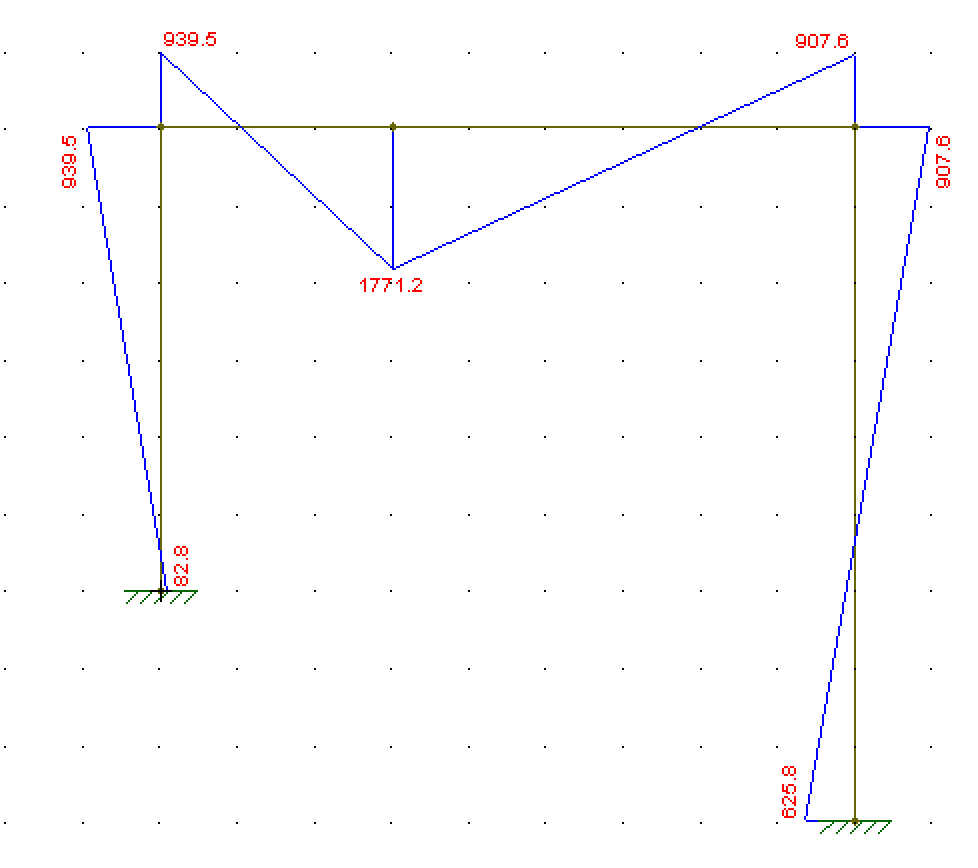
\includegraphics[width=0.53\textwidth]{ejUT3}
	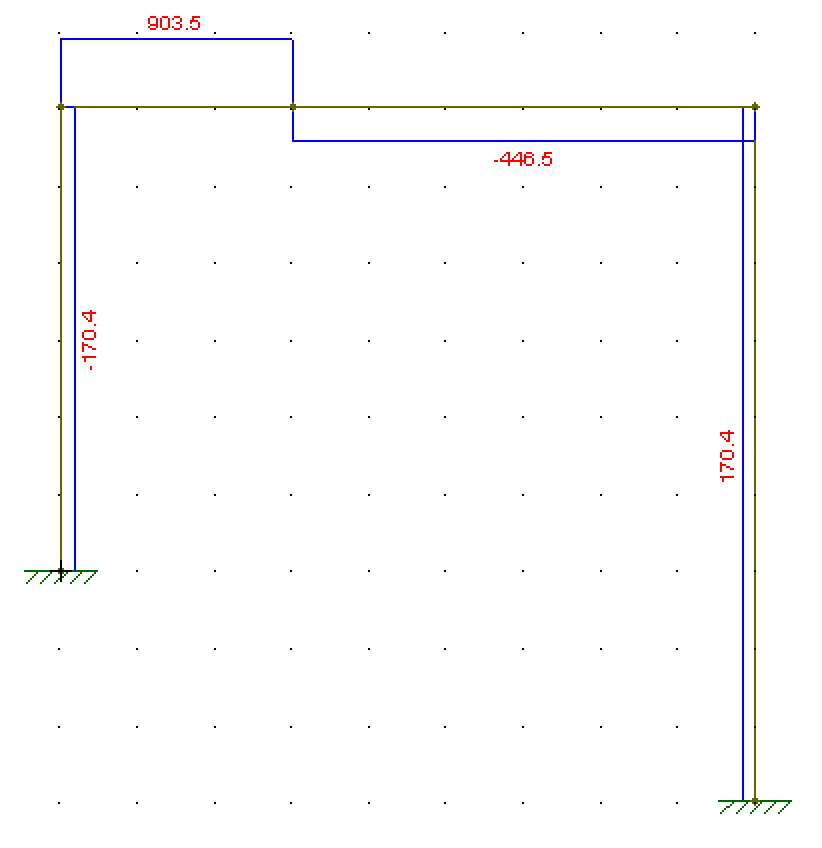
\includegraphics[width=0.45\textwidth]{ejUT3cort}
	\caption{Diagramas de momentos (izquierda) y cortante (derecha).}
	\label{fig:dia1}
\end{figure}

En la \autoref{fig:dia2} se muestran los diagramas de deformada y directas.
\begin{figure}[htb]
	\centering
	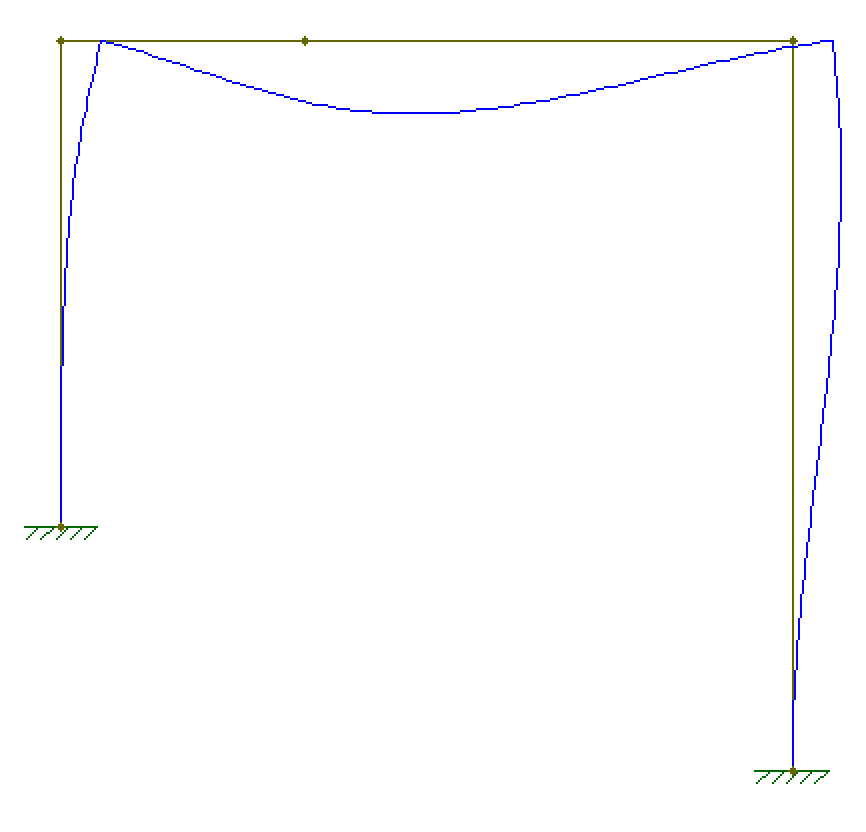
\includegraphics[width=0.45\textwidth]{ejUT3defor}
	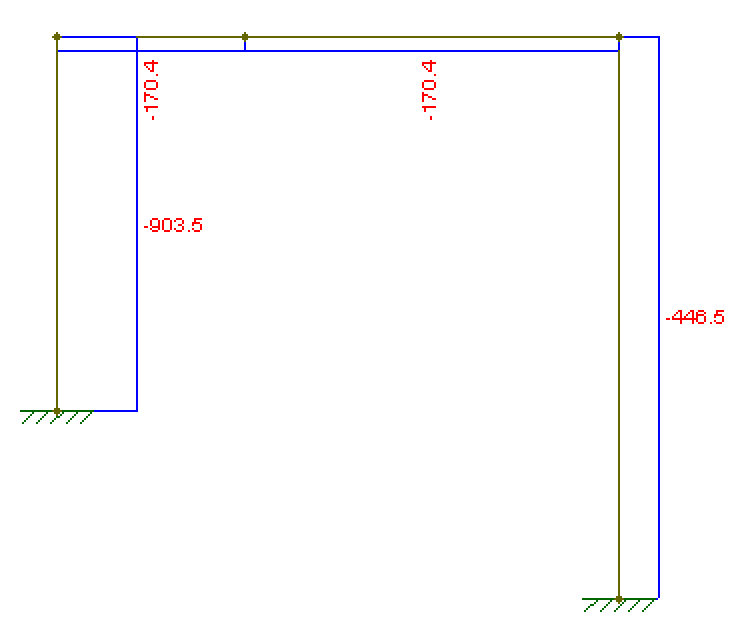
\includegraphics[width=0.53\textwidth]{ejUT3dire}
	\caption{Diagramas de deformada (izquierda) y directas (derecha).}
	\label{fig:dia2}
\end{figure}


\clearpage







\section{Métodos de análisis matricial/computacional}

En esta sección se presentan algunos desarrollos y métodos útiles para comprender el funcionamiento de las herramientas computacionales para el análisis de pórticos planos considerando deformación axial. %
%
Se utiliza un enfoque usualmente utilizado tanto en libros de resistencia de materiales \citep{Pilkey2002} como en libros orientados a métodos computacionales \citep{Onate2013}. %

Se considera una viga bajo las mismas hipótesis establecidas previamente, formada por un material elástico lineal de módulo de Young E sometida a esfuerzos de directa y momento tales que se produce una extensión y flexión. %
%
La expresión de la función de la deformación axial para un punto en $(x,y)$ es:
%
\begin{equation}
\varepsilon_x (x,y) = \varepsilon_G(x) - y \frac{\partial^2 v}{\partial x^2} (x),
\end{equation}
considerando los ejes tal como se muestra en la Figura~\ref{fig:viga3d}. %
%%	
Por otra parte, la tensión axial está dada por:
%
\begin{equation}
\sigma_x (x,y) = E \varepsilon_x(x,y) = E \varepsilon_G(x) - E y \frac{\partial^2 v}{\partial x^2} (x).
\end{equation}

Utilizando estas expresiones y realizando un procedimiento similar al de la Unidad Temática anterior se obtendrán las relaciones entre fuerzas y desplazamientos dadas por el Método de los Desplazamientos en flexión compuesta.

\subsection{Relaciones fuerzas-desplazamiento}

Se considera un elemento de viga con sección transversal uniforme de área $A$ e inercia $I$ de largo $\ell$. %
%
Se considera sometido a fuerzas nodales axiales y transversales y momentos nodales como es mostrado en la Figura~\ref{fig:ejeviga}. %
%
En dicha figura se muestra el eje de la viga en la configuración de referencia con las fuerzas aplicadas y la configuración deformada con los desplazamientos y giros nodales indicados de acuerdo a la convención de signos 2 (ver Figura~\ref{fig:conve}). %
%
\begin{figure}[htb]
	\setlength{\unitlength}{0.8\textwidth}
	\centering
	\def\svgwidth{0.8\textwidth}
	\input{figs/UT4/eje_viga_deformada.pdf_tex}
	\caption{Esquemas de viga: (a) eje de viga en configuración de referencia (línea punteada) y eje de viga deformada (línea continua), (b) eje de viga de referencia con fuerzas aplicadas.}
	\label{fig:ejeviga}
\end{figure}

El desplazamiento de cada nodo de la viga es interpolado a partir de sus desplazamientos y giros nodales, representados en forma vectorial como:
%
\begin{equation}
\bfu = [ u_1, v_1, \theta_1, u_2, v_2, \theta_2 ]^T.
\end{equation}

La energia potencial de deformación de la viga está dada por la expresión:
%
\begin{equation}
\Pi_{int}(\bfu) = \frac{1}{2} \int_{\Omega} E \varepsilon_x (x)^2 \dif V = \frac{1}{2} \int_{\ell} \int_{A} E \left( \varepsilon_G(x) -y \frac{\partial ^2 v}{\partial x^2}(x) \right)^2 \dif A \dif x .
\end{equation}

%
Desarrollando se tiene:
%
\begin{eqnarray}
\Pi_{int}(\bfu) 
&=& \frac{1}{2} \int_{\ell} \int_{A} E \left( \varepsilon_G(x)  \right)^2 \dif A \dif x \nonumber\\
\dots &-&             \int_{\ell} \int_{A} E y \varepsilon_G(x)  \frac{\partial ^2 v}{\partial x^2}(x)  \dif A \dif x \nonumber\\
\dots &+&             \frac{1}{2} \int_{\ell} \int_{A} E y^2 \left(  \frac{\partial ^2 v}{\partial x^2}(x) \right)^2 \dif A \dif x ,
\end{eqnarray}
%
y usando que el origen del sistema de coordenadas es el baricentro de la sección y siendo que la sección transversal es uniforme, se tiene:
%
\begin{equation}
\Pi_{int}(\bfu)  =
\underbrace{ \frac{1}{2} \int_{\ell} \int_{A} E \left( \varepsilon_G(x)  \right)^2 \dif A \dif x }_{\text{axial}}
+  
\underbrace{ \frac{1}{2} \int_{\ell} \int_{A} E y^2 \left(  \frac{\partial ^2 v}{\partial x^2}(x) \right)^2 \dif A \dif x}_{\text{flexión}}.
\end{equation}

En esta expresión fueron definidos los términos de energía de deformación por esfuerzo axial y por esfuerzo de flexión. %
%
Considerando que no existen cargas axiales aplicadas en el tramo del elemento se tiene que la deformación axial del baricentro está dada por:
%
\begin{equation}
\varepsilon_G(x) = \frac{u_2 - u_1}{\ell},
\end{equation}
%
a lo largo de todo el elemento. %
Esto permite expresar las energías en función de los desplazamientos nodales:
%
\begin{equation}
\Pi_{int}(\bfu) = \Pi_{int,\text{axial}}(u_1,u_2) + \Pi_{int,\text{flexión}}(v_1,\theta_1,v_2,\theta_2)
\end{equation}
%
donde la energía de deformación por esfuerzos axiales está dada por:
%
\begin{equation}\label{eqn:Uaxial}
\Pi_{int,\text{axial}}(u_1,u_2) = \frac{1}{2} \frac{E A}{\ell} (u_2 - u_1)^2 
\end{equation}
%
y la energía de deformación por exfuerzos de flexión está dada por:
%
\begin{equation} \label{eqn:Uflex}
\Pi_{int,\text{flexión}} (v_1,\theta_1,v_2,\theta_2) = \frac{1}{2} E I \int_{\ell} \left( \frac{\partial ^2 v}{\partial x^2}(x,v_1,\theta_1,v_2,\theta_2) \right)^2\dif x .
\end{equation}
Nuevamente se recuerda que se está usando que la sección transversal es uniforme.

La energía potencial de las fuerzas externas puede escribirse como:
\begin{equation}
\Pi_{ext} (\bfu) = - \bfu^T \bff
\end{equation}
%
donde $\bff$ es el vector columna de las fuerzas nodales, dado por:
%
\begin{equation}
\bff = [F_{x,1},F_{y,1},M_{1}, F_{x,2},F_{y,2},M_{2} ]^T.
\end{equation}


Se puede obtener por lo tanto la expresión de la energía potencial total:
%
\begin{equation}
\Pi (\bfu) =  \Pi_{int,\text{axial}}(u_1,u_2) + \Pi_{int,\text{flexión}}(v_1,\theta_1,v_2,\theta_2) - \bfu^T \bff
\end{equation}
%
y aplicar las condiciones dadas por el primer teorema de Castigliano:
%
\begin{eqnarray}
\frac{\partial \Pi_{int} }{\partial u_1} = \frac{EA}{\ell} (u_1 - u_2) &=& F_{x,1} \\
%
\frac{\partial \Pi_{int} }{\partial v_1} = EI \left( \dfrac{12}{\ell^{3}} v_1 + \dfrac{6}{\ell^{2}} \theta_1 - \dfrac{12}{\ell^{3}} v_2 + \dfrac{6}{\ell^{2}} \theta_2 \right)  &=& F_{y,1} \\
%
\frac{\partial \Pi_{int} }{\partial \theta_1} = EI \left( \frac{6}{\ell^2} v_1 +  \frac{4}{\ell} \theta_1 - \frac{6}{\ell^2} v_2   + \frac{2}{\ell} \theta_2 \right) &=& M_1 \\
\frac{\partial  \Pi_{int} }{\partial u_2} = \frac{EA}{\ell} (-u_1 + u_2) &=& F_{x,2} \\
%
\frac{\partial \Pi_{int} }{\partial v_2} = EI \left( -\dfrac{12}{\ell^{3}} v_1 - \dfrac{6}{\ell^{2}} \theta_1 +\dfrac{12}{\ell^{3}} v_2 - \dfrac{6}{\ell^{2}} \theta_2 \right) &=& F_{y,2} \\
%
\frac{\partial \Pi_{int} }{\partial \theta_2} = EI \left( \dfrac{6}{\ell^{2}} v_1 + \dfrac{2}{\ell} \theta_1 - \dfrac{6}{\ell^{2}} v_2 + \dfrac{4}{\ell}  \theta_2 \right) &=& M_2.
\end{eqnarray}

Estas condiciones representan la consideración conjunta de las condiciones vistas para la flexión en la Unidad Temática 3 y la deformación axial en la Unidad Temática 2.
%
Esta relación entre desplazamientos nodales y fuerzas puede ser planteada en forma matricial como:
%
\begin{equation}\label{eqn:eqrig}
\bfK \bfu = \bff,
\end{equation}
%
donde la matriz $\bfK$ es la llamada matriz de rigidez:
%
\begin{equation}
\bfK = \left[
\begin{matrix}
\dfrac{EA}{\ell} & 0 & 0 & - \dfrac{EA}{\ell} & 0 & 0 \\[3mm]
%
0 &  12 \dfrac{EI}{\ell^{3}} & 6 \dfrac{EI}{\ell^{2}} &  0& -12 \dfrac{EI}{\ell^{3}} & 6 \dfrac{EI}{\ell^{2}} \\[3mm]
0 &  6 \dfrac{EI}{\ell^{2}} & 4 \dfrac{EI}{\ell} & 0& -6 \dfrac{EI}{\ell^{2}} & 2 \dfrac{EI}{\ell} \\[3mm]
-\dfrac{EA}{\ell} & 0 & 0 &  \dfrac{EA}{\ell} & 0 & 0 \\[3mm]
%
0 &  -12 \dfrac{EI}{\ell^{3}} & -6 \dfrac{EI}{\ell^{2}} &0&  12 \dfrac{EI}{\ell^{3}} & -6 \dfrac{EI}{\ell^{2}} \\[3mm]
0 &  6 \dfrac{EI}{\ell^{2}} & 2 \dfrac{EI}{\ell} & 0 & -6 \dfrac{EI}{\ell^{2}} & 4 \dfrac{EI}{\ell} \\[3mm]
\end{matrix}
\right].
\end{equation}


Es importante destacar que la matriz de rigidez es simétrica, lo que puede ser justificado por el hecho de que la función de energía potencial total es una función de tipo $C^2$ y que la matríz $\bfK$ es la hesiana  de dicha función. %

Por otra parte también se destaca que la matriz $\bfK$ tiene valores propios nulos con sus correspondientes vectores propios asociados. %
(pertenecientes al subespacio asociado al valor propio cero $S_0$). %
%
Esto quiere decir que existen movimientos (dados por los vectores de desplazamientos en dicho subespacio) que se corresponden con fuerzas nodales nulas, por lo tanto estos movimientos no introducen deformaciones o tensiones en el elemento. %
%
Dicho de otra forma, estos movimientos serán los movimientos de cuerpo rígido de la viga. %
%
Estos movimientos son 3 por lo que es necesario eliminar tres grados de libertad (a través de las condiciones de contorno) para obtener una matriz reducida con valores propios positivos y por lo tanto invertible. %
%
De esta forma la solución del sistema es única.

\subsection{Sistemas de coordenadas y análisis matricial}

Para encontrar la relación entre desplazamientos y fuerzas nodales en problemas de pórticos donde los ejes de los elementos que concurren a un nodo no coinciden, es útil definir un sistema de coordenadas global de la misma forma en que fue realizado para reticulados planos.
%

En el caso de pórticos el cambio de base se aplica a los desplazamientos nodales, mientras que los giros se mantienen en el mismo versor de referencia. %
%
La matriz de cambio de base esta dada por
%
\begin{equation}
\bfR^e = 
\left[
\begin{matrix}
c & -s & 0 & 0 &  0 & 0 \\
s & c & 0 & 0 &  0 & 0\\
0 & 0 &1 & 0 &  0 & 0\\
0 & 0 &0  &   c & -s& 0\\
0 & 0 &0  &  s & c & 0\\
0 & 0 &0 & 0 &  0 & 1\\
\end{matrix}
\right]
\qquad
\bfu^e = \bfR^e \bfu^e_L
\end{equation}
%
donde $c=\cos(\alpha^e)$ y $s=\sin(\alpha^e)$ y $\alpha^e$ es el ángulo medido positivo antihorario desde el eje global al local. %
%
La Ecuación~\eqref{eqn:eqrig} fue desarrollada en coordenadas locales utilizando la notación $\bfu$, la cual en el caso de sistemas coordenadas locales y globales correspondería a los ejes locales, por lo que debería ser escrita como
\begin{equation}
\bfK_L \bfu_L = \bfF_L.
\end{equation}
%
La matriz de rigidez en coordenadas globales está dada por:
\begin{equation}
\bfK^e_G = \bfR^e \bfK^e_L (\bfR^e)^T
\end{equation}

%
El sistema global obtenido luego de realizado el ensamblado es denotado por:
\begin{equation}
\bfK_G \bfu = \bfF_G.
\end{equation}
donde $\bfF_G$ es el vector de fuerzas externas nodales en coordenadas globales.

La determinación de desplazamientos a través del ensamblado de un sistema de ecuaciones lineales es llamado Análisis Matricial dado que se realiza a través del ensamblado e inversión de matrices de dimensiones considerables. %
%
La aplicación de este método para estructuras con cargas nodales es equivalente al MEF utilizando elementos de pórtico (\textit{frame} en inglés) \citep{Onate2013}, procedimiento utilizado por la mayoría de los programas computacionales de determinación de solicitaciones.

\subsection{Apoyos elásticos}

Para la resolución mediante análisis matricial o  de forma computacional, las fuerzas introducidas por los resortes pueden ser consideradas a través de una matriz de rigidez para cada elemento (en coordenadas globales):
\begin{equation}
\bfK_S^e = 
\left[
\begin{matrix}
k_{u1} & 0 & 0 & 0 &  0 & 0 \\
0 & k_{v1} & 0 & 0 &  0 & 0\\
0 & 0 &k_{\theta1} & 0 &  0 & 0\\
0 & 0 &0  &   k_{u2} & 0& 0\\
0 & 0 &0  &  0 & k_{v2} & 0\\
0 & 0 &0 & 0 &  0 & k_{\theta2}\\
\end{matrix}
\right]
\end{equation}
que puede ser ensamblada y sumada a la matriz de rigidez global, obteniendo un sistema dado por
%
\begin{equation}
\left(\bfK_G + \bfK_S \right) \bfu = \bfF_G.
\end{equation}

\subsection{Comparación de energías de deformación}

Tal como fue visto en la Unidad Temática 3, para la aplicación de métodos analíticos como el método de Slope-deflection, es usual considerar que la energía de deformación por directa es despreciable respecto a la de flexión. Esto permite eliminar algunas incógnitas cinemáticas. %

Esta hipótesis es adecuada si se cumple:
%
\begin{equation}
\Pi_{int,\text{axial}} \ll \Pi_{int,\text{flexión}}
\end{equation}
%
lo que es equivalente a:%
%
\begin{equation}
\frac{1}{2} \int_{0}^{\ell} E A  \varepsilon_G^2 \dif x \ll \frac{1}{2} \int_{0}^{\ell} EI \left( \frac{\partial^2 v}{\partial x^2}\right)^2 \dif x
\end{equation}
usando las expresiones obtenidas en la unidad temática 3: 
\begin{equation}
\varepsilon_G(x) = \frac{	N (x) }{E A}
\quad
\text{y}
\quad
\frac{\partial^2 v}{\partial x^2}(x) = \frac{	M (x) }{E I} ,
\end{equation}
se tiene que esa condición es equivalente a 
%
\begin{equation}
\int_{0}^{\ell} \frac{	N (x)^2 }{E A} \dif x \ll \int_{0}^{\ell} \frac{	M (x)^2 }{E I}  \dif x.
\end{equation}



\subsection{Método de Elementos Finitos}

El Método de Elementos Finitos (MEF) puede también ser considerado un método de desplazamientos ya que las incógnitas principales son desplazamientos y giros. %
%
Por otra parte, el enfoque del método permite obtener las ecuaciones que gobiernan la deformación de diversos elementos estructurales \citep{Onate2013}.

Se pueden enumerar algunas diferencias centrales respecto a los métodos analíticos.
%
\begin{itemize}
	\item Para cargas puntuales aplicadas en el tramo, en el MEF se suele dividir el elemento de viga en dos elementos, agregando un nodo en el punto de aplicación de la carga. Esto aumenta la cantidad de variables, lo cual no es relevante dado que el sistema lineal es resuelto numéricamente, y también simplifica la implementación del método.
	%
	\item Las cargas distribuidas suelen ser consideradas discretizando el elemento en un número apropiado de elementos finitos agregando nodos intermedios y por lo tanto más incógnitas del problema. De esta forma se pueden calcular los diagramas de solicitaciones aproximados de forma directa. % 
	Se debe también tener en cuenta que las solicitaciones no necesariamente serán exactas dentro del dominio de cada elemento, dado que existen aproximaciones por la interpolación considerada.
	%
	\item En el MEF es posible automatizar la verificación de estabilidad del esquema básico estructural considerado, a través del análisis de los valores propios de la matriz de rigidez ensamblada y con las condiciones de contorno aplicadas. %
	%
	Esto permite automatizar esa verificación, considerada muy importante al obtener solicitaciones de estructuras de grandes dimensiones \citep{Kannan2014}. 
\end{itemize}

En este curso no se mencionan aspectos sobre la convergencia de las soluciones al aumentar la cantidad de elementos finitos, el estudiante interesado puede consultar \citep{Hughes1987a}.

El ONSAS es un ejemplo de herramienta numérica basada en el método de los elementos finitos.

%
%\subsubsection{Comparación MSD, MEF y soluciones analíticas}
%
%Los métodos MSD y MEF son derivados a partir de las mismas ecuaciones y ambos son métodos de desplazamientos. %
%Sin embargo se puede decir que una diferencia a tener en cuenta es la cantidad de incógnitas a determinar. %
%%
%En el MSD las cargas en el tramo son incluidas a través del vector de fuerzas nodales mientras que en el MEF se suelen agregar nodos intermedios. %
%% 
%
%








\section{Ejercicios}
\setcounter{ejercicio}{0}

En cada ejercicio o estructura descrita a continuación, se pide:
%
\begin{enumerate}
  \item Identificar la mínima cantidad de incógnitas a hallar para obtener las solicitaciones de la estructura mediante el método de Slope Deflection.
  \item  Encontrar las ecuaciones que permiten resolver dichas incógnitas.
  \item  Calcular reacciones y trazar diagramas de solicitaciones.
  \item  Modelar las estructuras en un programa computacional y comparar resultados.
\end{enumerate}

\ejercicio

La viga de madera de la figura ($E=10$ GPa), compuesta por una escuadría de $20$ cm $\times$ $40$ cm.

\begin{center}
	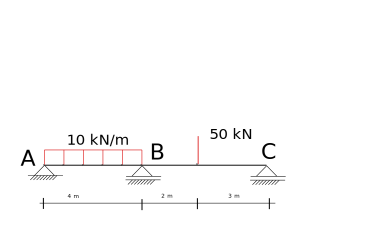
\includegraphics[width=0.9\linewidth]{UT3ej1}
\end{center}


\ejercicio

La estructura de acero de la figura ($E=210$ GPa), compuesta por una viga (ABC) formada por 1 PNI28 y un pilar (BD) formada por un perfil PNI22.

\begin{center}
	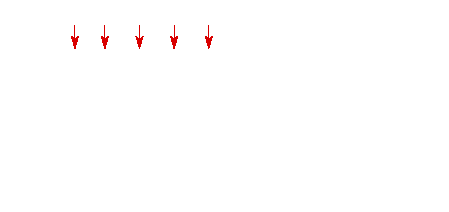
\includegraphics[width=0.6\linewidth]{UT3ej2}
\end{center}


\ejercicio

La estructura de acero ($E=210$ GPa) compuesta por una viga (ABC), dos pilares (AD y BE) y un tensor (BD), cuya sección es 1PNI18.

\begin{center}
	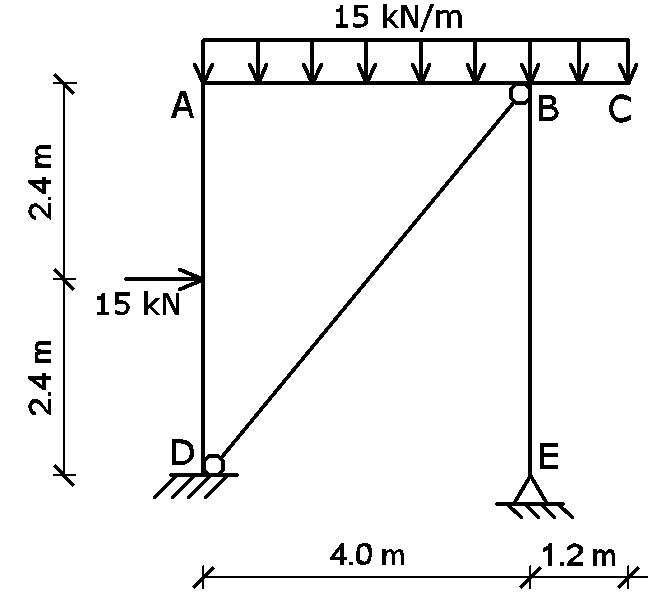
\includegraphics[width=0.5\linewidth]{UT3ej3}
\end{center}

\ejercicio

En la estructura de hormigón de la figura (E=25 GPa) los pilares son de 20x30 cm mientras que la viga es de 15x40 cm. 

\begin{center}
	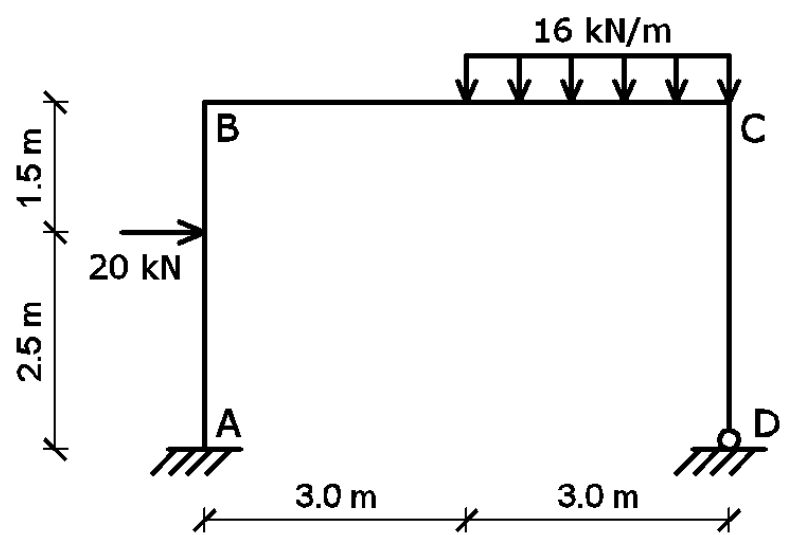
\includegraphics[width=0.65\linewidth]{UT3ej4}
\end{center}


\ejercicio

En la estructura de acero de la figura (E=210 GPa), las barras BD, CF y DE están conformadas por 2PNC24 soldados ([]), mientras que la barra AB está compuesta por 1PNI20. 


\begin{center}
	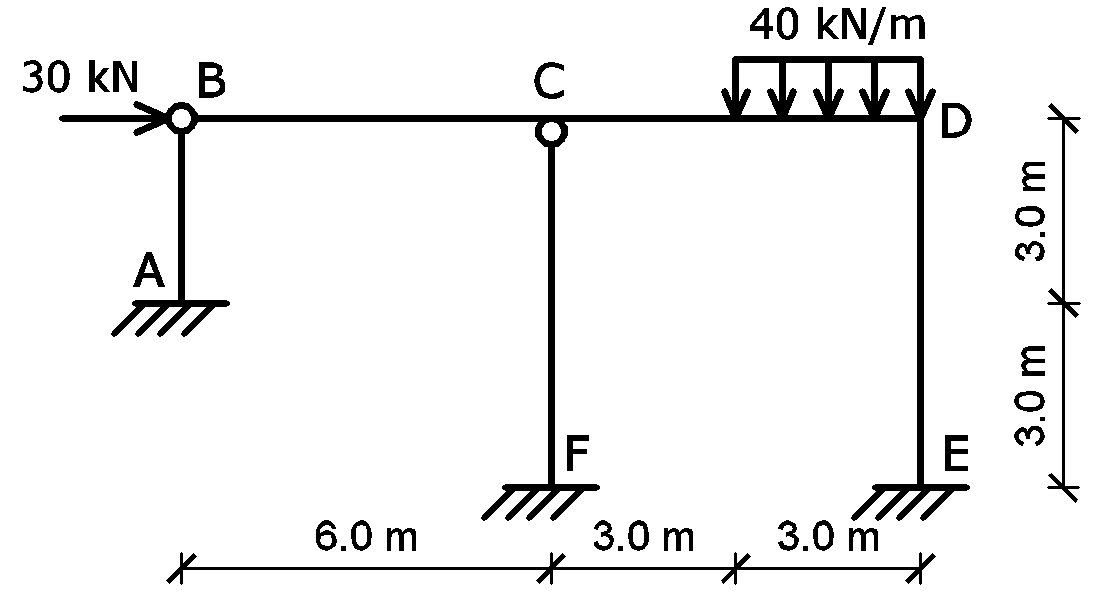
\includegraphics[width=0.75\linewidth]{UT3ej5}
\end{center}



\ejercicio 

En la estructura de hormigón de la figura (E=30 GPa) las secciones son rectangulares de 12x30 cm. 

\begin{center}
	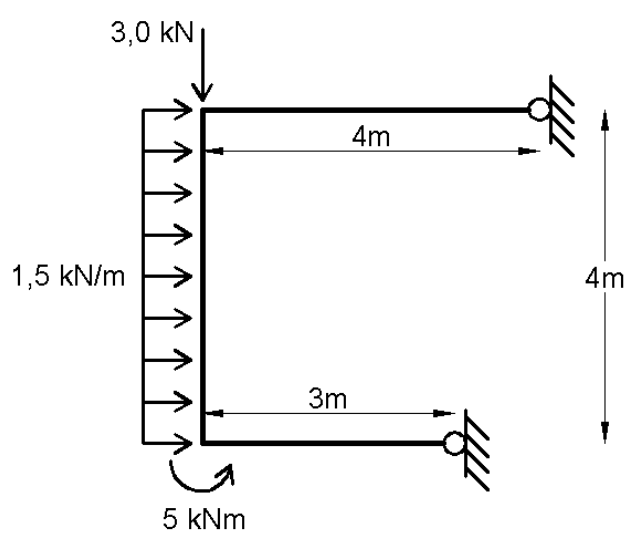
\includegraphics[width=0.6\linewidth]{UT3ej6}
\end{center}


\ejercicio


Sean las siguientes estructuras conformadas por barras de \textbf{EI}=cte y de longitud \textbf{L} sometidas a un desplazamiento impuesto $\Delta$. Se pide calcular los momentos flectores en los empotramientos.


\begin{center}
	\def\svgwidth{0.45\textwidth}
	a) \input{figs/UT3/UT3ejDespa.pdf_tex}
	\def\svgwidth{0.45\textwidth}
	b) \input{figs/UT3/UT3ejDespb.pdf_tex}
\end{center}
